% !TeX program = lualatex
% ================================================================
% Polish Parallel Text Version of ReadingScalesAndErrorIntervals
%
% Generated by the server using the following settings:
%
%   language            Polish (pol)
%   text direction      left to right
%   font                Noto Serif
%   fallback font       Noto Serif
%   built from          latex/worksheets/measures/metric/readingScalesAndErrorIntervals.tex
%   vocabulary key      latex/worksheets/measures/metric/readingScalesAndErrorIntervals/L2/pol/readingScalesAndErrorIntervals_polishKey.tex
%   tier 3 vocabulary   green   RGB 0 128 0
%   English text        black   RGB 0 0 0
%   Polish text         purple  RGB 112 48 160
%   layout macros       version 3
%
% Please don't edit any information in this comment block - the server
% compares it against the current settings and rebuilds this file when
% they differ, so changes here would be overwritten. However, feel free
% to make updates to the LaTeX below if you want to edit it.
% ================================================================

\documentclass[11pt,a4paper]{article}
% ================================================================
% Copied from the English sheet this was translated from, so that
% anything it sets up for itself still works here
% ================================================================
\usepackage[a4paper,top=10mm,bottom=10mm,left=14mm,right=14mm]{geometry}
\usepackage[T1]{fontenc}
\usepackage{amsmath}
\usepackage{amssymb}
\usepackage{enumitem}
\usepackage{multicol}
\usepackage{array}
\usepackage{tikz}
\usepackage[most]{tcolorbox}
\usetikzlibrary{arrows.meta,calc,decorations.pathreplacing}

% ================================================================
% Reading scales and error intervals.
%
% A Year 7 sheet on how accurate a measurement read from a scale is.
% Part 1 shows enlarged views of the scales on rulers, a metre rule,
% a measuring jug, a measuring cylinder, kitchen scales, luggage
% scales and a river depth gauge. Pupils work out what one gap
% between two ticks is worth, then round each measurement to the
% nearest tick. The scaffold under each picture fades as the part
% goes on.
%
% Part 2 introduces the lower bound, the upper bound and the error
% interval of a reading. The worked example is a metre rule marked
% in centimetres, which is accurate to plus or minus 0.5 cm. It is
% followed by the same layout with gaps, then the same layout with
% fewer gaps, then the readings from Part 1 again with only the
% inequality as a frame, and then a table of measurements with no
% frame. Part 3 has reverse problems, questions about whether a
% reading can be trusted, a scale for pupils to design, and ends
% with an open task about an instrument of their own choosing.
%
% The sheet is written on and is four sides of A4. The \newpage
% commands are placed so that no question is split across a page.
%
% In every picture the end of the object, the surface of the liquid
% or the pointer is drawn 0.3 or 0.7 of a gap past a tick, so that
% the nearest tick is clear and a reading is never a halfway case.
% Each picture is drawn from the value in the comment beside it, so
% a reading can be changed by changing one coordinate.
%
% Readings: Q1 14 cm, Q2 76 cm, Q3 340 ml, Q4 36 ml, Q5 440 g,
% Q6 5.4 cm, Q7 23.6 kg, Q8 1.3 m.
% ================================================================

\pagestyle{empty}
\setlength{\parindent}{0pt}
\setlength{\parskip}{3pt}
\setlength{\multicolsep}{3pt}
\setlength{\columnsep}{14pt}
\setlist[enumerate,1]{label=\textbf{Q\arabic*.}, leftmargin=*, itemsep=7pt, topsep=3pt, parsep=2pt}
\setlist[enumerate,2]{label=(\alph*), leftmargin=*, itemsep=5pt, topsep=3pt, parsep=1pt}
\newcolumntype{C}[1]{>{\centering\arraybackslash}m{#1}}

\newcommand{\ansline}[1][2.2cm]{\underline{\hspace{#1}}}
% A full-width line to write an explanation on.
\newcommand{\wline}{\par\vspace{15pt}\noindent\rule{\linewidth}{0.4pt}}
% The strut that sets the height of a table row to be written in.
\newcommand{\rowstrut}{\rule[-3.5mm]{0pt}{9.5mm}}

% The questions in Part 1 sit side by side in minipages, so they are
% numbered by hand with this counter. The lists in Parts 2 and 3
% carry on from it.
\newcounter{qn}
\newcommand{\q}{\refstepcounter{qn}\textbf{Q\theqn.}\ }

% A worked example: the method shown in full before it is practised.
% The boxes are drawn in pale tints, with a pale title bar, so that
% the printed sheet uses little toner.
\newtcolorbox{wex}[1]{colback=blue!2,colframe=blue!30,boxrule=0.6pt,
  colbacktitle=blue!8,coltitle=blue!50!black,
  left=6pt,right=6pt,top=4pt,bottom=5pt,
  title={\bfseries\small Worked example: #1},fonttitle=\small,
  toptitle=1pt,bottomtitle=1pt}

% The idea a part is built on, stated once and boxed.
\newtcolorbox{keyidea}{colback=orange!3,colframe=orange!35,boxrule=0.6pt,
  left=6pt,right=6pt,top=4pt,bottom=4pt}

% The section headings, kept tight so the parts do not eat the page.
\newcommand{\parttitle}[2]{%
  \vspace{1pt}
  {\color{blue!45!black}\rule{\linewidth}{1pt}}\\[1pt]
  {\large\bfseries Part #1: #2}\\[-6pt]
  {\color{blue!45!black}\rule{\linewidth}{0.4pt}}
  \par\vspace{-3pt}}

% ----------------------------------------------------------------
% Close-up pictures of scales.
%
% Each picture is clipped to a rounded window between \zoomclip and
% \zoomframe, and a small magnifying glass on the corner of the
% window shows that the view is enlarged.
\tikzset{
  tick/.style={line width=0.5pt},
  ticklab/.style={font=\scriptsize, inner sep=1.5pt},
  scalebody/.style={fill=yellow!7, draw=black!60, line width=0.5pt},
  water/.style={fill=blue!13},
  surface/.style={blue!60!black, line width=0.9pt},
}
\newcommand{\zoomclip}[4]{%
  \def\zxa{#1}\def\zya{#2}\def\zxb{#3}\def\zyb{#4}%
  \begin{scope}\clip[rounded corners=6pt] (#1,#2) rectangle (#3,#4);}
\newcommand{\zoomframe}{%
  \end{scope}
  \draw[black!55, line width=0.9pt, rounded corners=6pt] (\zxa,\zya) rectangle (\zxb,\zyb);
  \draw[black!55, line width=1.8pt, line cap=round] ($(\zxb,\zyb)+(0.14,0.14)$) -- ++(0.22,0.22);
  \draw[black!55, line width=0.8pt, fill=white] (\zxb,\zyb) circle (0.19);}

% Ticks along the top edge of a horizontal scale, hanging down from
% y = 0, with tick i at x = i times the gap.
% \hticks{first i}{last i}{cm per gap}{label every}{longer tick every}{value at i=0}{value per gap}
\newcommand{\hticks}[7]{%
  \foreach \i in {#1,...,#2}{%
    \pgfmathtruncatemacro{\islab}{ifthenelse(mod(\i,#4)==0,1,0)}%
    \pgfmathtruncatemacro{\ismid}{ifthenelse(mod(\i,#5)==0,1,0)}%
    \ifnum\islab=1
      \draw[tick] ({\i*(#3)},0) -- ++(0,-0.5);
      \pgfmathsetmacro{\val}{#6+\i*(#7)}%
      \node[ticklab,below] at ({\i*(#3)},-0.5) {\pgfmathprintnumber{\val}};
    \else\ifnum\ismid=1
      \draw[tick] ({\i*(#3)},0) -- ++(0,-0.36);
    \else
      \draw[tick] ({\i*(#3)},0) -- ++(0,-0.22);
    \fi\fi}}

% Ticks up the side of a vertical scale, pointing right from x = 0,
% with tick i at y = i times the gap. A negative gap makes the values
% increase downwards.
% \vticks{first i}{last i}{cm per gap}{label every}{longer tick every}{value at i=0}{value per gap}{unit}
\newcommand{\vticks}[8]{%
  \foreach \i in {#1,...,#2}{%
    \pgfmathtruncatemacro{\islab}{ifthenelse(mod(\i,#4)==0,1,0)}%
    \pgfmathtruncatemacro{\ismid}{ifthenelse(mod(\i,#5)==0,1,0)}%
    \ifnum\islab=1
      \draw[tick] (0,{\i*(#3)}) -- ++(0.75,0);
      \pgfmathsetmacro{\val}{#6+\i*(#7)}%
      \node[ticklab,right] at (0.75,{\i*(#3)}) {\pgfmathprintnumber{\val}\,#8};
    \else\ifnum\ismid=1
      \draw[tick] (0,{\i*(#3)}) -- ++(0.55,0);
    \else
      \draw[tick] (0,{\i*(#3)}) -- ++(0.38,0);
    \fi\fi}}

% A pencil lying along the top of a ruler, with its tip at x = #1.
\newcommand{\pencil}[1]{%
  \filldraw[fill=yellow!35, draw=black!70] (-3,0.05) rectangle ({#1-1.0},0.59);
  \draw[black!35] (-3,0.32) -- ({#1-1.0},0.32);
  \filldraw[fill=orange!15, draw=black!70] ({#1-1.0},0.05) -- (#1,0.32) -- ({#1-1.0},0.59) -- cycle;
  \fill[black!65] ({#1-0.3},0.239) -- (#1,0.32) -- ({#1-0.3},0.401) -- cycle;}

% Part 1 layouts. A horizontal picture goes between the question and
% its answer lines. A tall picture goes to the left, with the
% question and answer lines beside it.
\newcommand{\hcell}[3]{%
  \begin{minipage}[t]{0.485\linewidth}
  #1\par\smallskip
  {\centering #2\par}\smallskip
  #3
  \end{minipage}}
\newcommand{\vcell}[3]{%
  \begin{minipage}[t]{0.485\linewidth}
  \begin{minipage}[t]{3.95cm}\vspace{0pt}#2\end{minipage}\hfill
  \begin{minipage}[t]{\dimexpr\linewidth-4.15cm\relax}\vspace{0pt}\raggedright #1\par\medskip #3\end{minipage}
  \end{minipage}}

% ----------------------------------------------------------------
% A number line for an error interval: three ticks one gap apart,
% then any extra drawing (the interval itself in the worked example).
\newcommand{\numline}[4]{%
  \begin{tikzpicture}[x=2.3cm, baseline=(current bounding box.north)]
  \draw[line width=0.7pt, {Stealth[length=5pt]}-{Stealth[length=5pt]}] (-0.4,0) -- (2.4,0);
  \foreach \x/\l in {0/#1,1/#2,2/#3}{%
    \draw[tick] (\x,0.15) -- (\x,-0.15);
    \node[ticklab,below] at (\x,-0.17) {\l};}
  #4
  \end{tikzpicture}}

% Characters this language's font has not got are borrowed from another,
% rather than being silently dropped - see docs/translated-sheet-latex.md
\directlua{%
  if luaotfload and luaotfload.add_fallback then
    luaotfload.add_fallback("eallatinfallback",
      { "Noto Serif:mode=harf;" })
  else
    tex.error("this luaotfload is too old to register a fallback font")
  end
}
\usepackage[english]{babel}
\babelprovide[import]{polish}
\babelfont[polish]{rm}[Renderer=Harfbuzz, BoldFont={Noto Serif}, ItalicFont={Noto Serif}, BoldItalicFont={Noto Serif}, RawFeature={fallback=eallatinfallback}]{Noto Serif}
\babelfont[polish]{sf}[Renderer=Harfbuzz, BoldFont={Noto Serif}, ItalicFont={Noto Serif}, BoldItalicFont={Noto Serif}, RawFeature={fallback=eallatinfallback}]{Noto Serif}
\newcommand{\ealtext}[1]{\foreignlanguage{polish}{#1}}
\newcommand{\ealtextblock}[1]{{\raggedright\foreignlanguage{polish}{#1}\par}}
% ================================================================
% EAL layout helpers
% ================================================================
\usepackage{xcolor}

\definecolor{ealkeycolour}{RGB}{0,128,0}
\definecolor{ealenglish}{RGB}{0,0,0}
\definecolor{ealtwocolour}{RGB}{112,48,160}

\newsavebox{\ealboxen}
\newsavebox{\ealboxtr}
\newlength{\ealglosswd}
\newlength{\ealglossraise}
\setlength{\ealglossraise}{1.15em}

% a tier 3 word, in English and in translation alike
\newcommand{\ealkey}[1]{\textcolor{ealkeycolour}{#1}}
\newcommand{\ealkeytr}[1]{\textcolor{ealkeycolour}{\ealtext{#1}}}

% One translated word above one English word. Built from kernel
% primitives, never a tabular, which would break wherever the sheet
% loads array, booktabs or tabularx. The box is as wide as the wider of
% the two, so a long translation pushes its neighbours aside instead of
% overlapping them, and it claims its full height so a table row or a
% TikZ node makes room for it.
\newcommand{\ealgloss}[2]{%
  \sbox{\ealboxen}{\ealkey{#1}}%
  \sbox{\ealboxtr}{\small\textcolor{ealtwocolour}{\ealtext{#2}}}%
  \setlength{\ealglosswd}{\wd\ealboxen}%
  \ifdim\wd\ealboxtr>\ealglosswd\setlength{\ealglosswd}{\wd\ealboxtr}\fi
  \leavevmode
  \makebox[\ealglosswd][c]{%
    \makebox[0pt][c]{\usebox{\ealboxen}}%
    \makebox[0pt][c]{\raisebox{\ealglossraise}{\usebox{\ealboxtr}}}%
  }%
}

% opens up line spacing around a block of glosses, so the raised
% translations sit clear of the line above
\newenvironment{ealglossed}{\par\linespread{2.1}\selectfont\ignorespaces}{\par}

% a whole translated sentence above its English counterpart. block level,
% so it does not belong inside a tabular cell
\newcommand{\ealpara}[2]{%
  \par\addvspace{0.5\baselineskip}%
  {\color{ealtwocolour}\ealtextblock{#1}}%
  \penalty200
  {\color{ealenglish}#2\par}%
  \addvspace{0.5\baselineskip}%
}

\begin{document}

\begin{center}
  {\Large\bfseries \ealpara{Czytanie skal i \ealkeytr{przedziałów błędu}}{Reading Scales and \ealkey{Error Intervals}}}
\end{center}
\vspace{6pt}

\ealpara{1 Czytanie skali do najbliższej \ealkeytr{kreski}}{}
\parttitle{1}{Reading a scale to the nearest \ealkey{tick}}

\ealpara{Znaki na skali pomiarowej nazywane są \ealkeytr{kreskami}. Każdy rysunek jest powiększonym widokiem części skali. Oblicz, ile warta jest jeden \ealkeytr{odstęp} między dwiema \ealkeytr{kreskami}, a następnie zapisz \ealkeytr{pomiar} do najbliższej \ealkeytr{kreski}.}{The marks on a measuring scale are called \textbf{\ealkey{ticks}}. Each picture is an enlarged view of part of a scale. Work out what one \ealkey{gap} between two \ealkey{ticks} is worth, then write the \ealkey{measurement} to the nearest \ealkey{tick}.}

\medskip
% Q1: tip of the pencil at 13.7 cm, so x = (13.7 - 9) * 1.1 = 5.17.
\ealpara{Ołówek mierzy się linijką oznaczoną w centymetrach. Drugi koniec ołówka jest przy 0\,cm. Końcówka znajduje się między ... cm a ... cm. Najbliżej jej do ... cm.}{}
\hcell{\q A pencil is measured with a ruler marked in centimetres. The other
end of the pencil is at 0\,cm.}
{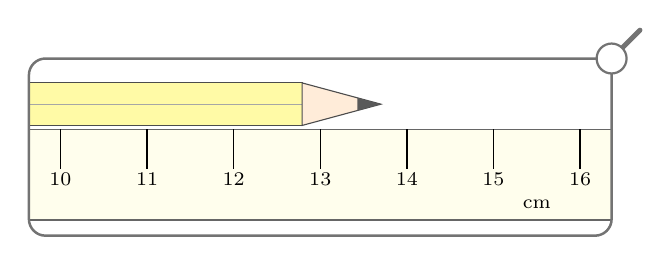
\begin{tikzpicture}
  \zoomclip{0.7}{-1.35}{8.1}{0.9}
    \filldraw[scalebody] (-1,-1.15) rectangle (9,0);
    \hticks{0}{8}{1.1}{1}{1}{9}{1}
    \node[ticklab] at (7.15,-0.95) {cm};
    \pencil{5.17}
  \zoomframe
\end{tikzpicture}}
{The tip is between \ansline[1.3cm]\,cm and \ansline[1.3cm]\,cm.\\[4pt]
It is nearest to \ansline[1.3cm]\,cm.}%
\hfill
% Q2: edge of the door at 76.3 cm, so x = 6.3 * 0.62 = 3.906.
\ealpara{Szerokość drzwi mierzy się metrem oznaczonym w centymetrach. Metr zaczyna się przy drugiej stronie drzwi. Jeden \ealkeytr{odstęp} między dwiema \ealkeytr{kreskami} jest wart ... cm. \ealkeytr{Odczyt} do najbliższej \ealkeytr{kreski}: ... cm.}{}
\hcell{\q The width of a door is measured with a metre rule marked in
centimetres. The metre rule starts at the other side of the door.}
{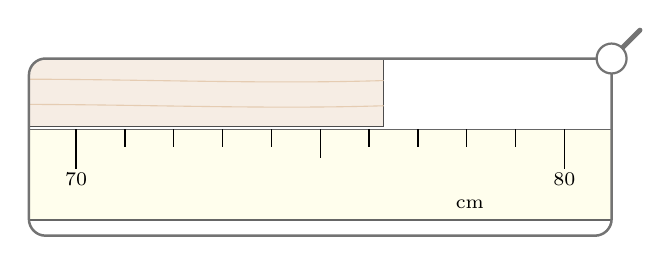
\begin{tikzpicture}
  \zoomclip{-0.6}{-1.35}{6.8}{0.9}
    \filldraw[fill=brown!14, draw=black!70] (-2,0.04) rectangle (3.906,2);
    \foreach \y in {0.3,0.62} \draw[brown!40] (-2,\y) .. controls (0,{\y+0.06}) and (2,{\y-0.06}) .. (3.906,\y);
    \filldraw[scalebody] (-2,-1.15) rectangle (8,0);
    \hticks{-2}{12}{0.62}{10}{5}{70}{1}
    \node[ticklab] at (5.0,-0.95) {cm};
  \zoomframe
\end{tikzpicture}}
{One \ealkey{gap} between two \ealkey{ticks} is worth \ansline[1.3cm]\,cm.\\[4pt]
\ealkey{Reading} to the nearest \ealkey{tick}: \ansline[1.3cm]\,cm.}

\vfill
% Q3: surface of the water at 334 ml, so y = (334 - 300) / 20 * 0.5 = 0.85.
\ealpara{Wodę wlewa się do dzbanka miarowego. Jeden \ealkeytr{odstęp} jest wart ... ml. \ealkeytr{Odczyt} do najbliższej \ealkeytr{kreski}: ... ml.}{}
\vcell{\q Water is poured into a measuring jug.}
{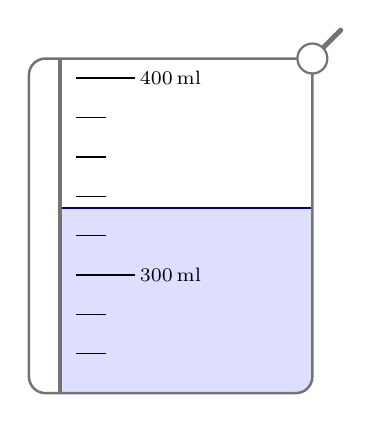
\begin{tikzpicture}[baseline=(current bounding box.north)]
  \zoomclip{-0.6}{-1.5}{3.0}{2.75}
    \fill[water] (-0.2,-3) rectangle (4,0.85);
    \draw[surface] (-0.2,0.85) -- (4,0.85);
    \draw[black!55, line width=1.4pt] (-0.2,-3) -- (-0.2,4);
    \vticks{-4}{6}{0.5}{5}{100}{300}{20}{ml}
  \zoomframe
\end{tikzpicture}}
{One \ealkey{gap} is worth \ansline[1.3cm]\,ml.\\[8pt]
\ealkey{Reading} to the nearest \ealkey{tick}:\\[4pt] \ansline[1.6cm]\,ml.}%
\hfill
% Q4: surface of the liquid at 36.6 ml, so y = (36.6 - 30) / 2 * 0.5 = 1.65.
\ealpara{Ciecz wlewa się do cylindra miarowego. Jeden \ealkeytr{odstęp} jest wart ... ml. \ealkeytr{Odczyt} do najbliższej \ealkeytr{kreski}: ... ml.}{}
\vcell{\q Liquid is poured into a measuring cylinder.}
{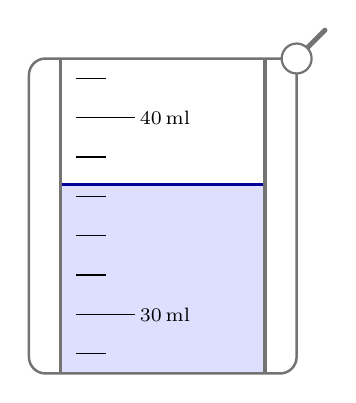
\begin{tikzpicture}[baseline=(current bounding box.north)]
  \zoomclip{-0.5}{-0.75}{2.9}{3.25}
    \fill[water] (-0.1,-2) rectangle (2.5,1.65);
    \draw[surface] (-0.1,1.65) -- (2.5,1.65);
    \draw[black!55, line width=1.2pt] (-0.1,-2) -- (-0.1,4);
    \draw[black!55, line width=1.2pt] (2.5,-2) -- (2.5,4);
    \begin{scope}[xshift=0.1cm]
      \vticks{-2}{7}{0.5}{5}{100}{30}{2}{ml}
    \end{scope}
  \zoomframe
\end{tikzpicture}}
{One \ealkey{gap} is worth \ansline[1.3cm]\,ml.\\[8pt]
\ealkey{Reading} to the nearest \ealkey{tick}:\\[4pt] \ansline[1.6cm]\,ml.}

\vfill
% Q5: needle at 437 g. Each 10 g is 4.6 degrees, with 450 g straight
% up, so the needle is at 90 + 1.3 * 4.6 = 95.98 degrees.
\ealpara{Mąkę waży się na wadze kuchennej. Jeden \ealkeytr{odstęp} jest wart ... g. \ealkeytr{Odczyt} do najbliższej \ealkeytr{kreski}: ... g.}{}
\hcell{\q Flour is weighed on kitchen scales.}
{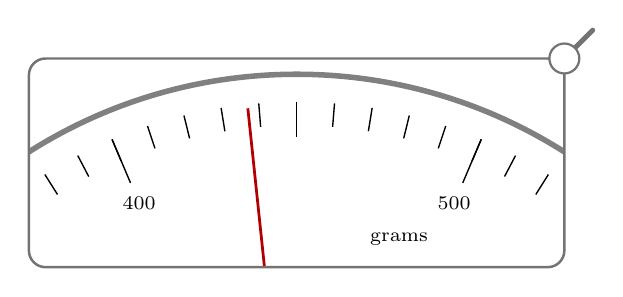
\begin{tikzpicture}
  \zoomclip{-3.4}{3.9}{3.4}{6.55}
    \draw[black!50, line width=2pt] (0,0) circle (6.35);
    \foreach \i in {-8,...,8} \draw[tick] ({90-4.6*\i}:6) -- ({90-4.6*\i}:5.7);
    \draw[tick] (90:6) -- (90:5.55);
    \foreach \i/\v in {-5/400,5/500}{%
      \draw[tick] ({90-4.6*\i}:6) -- ({90-4.6*\i}:5.4);
      \node[ticklab] at ({90-4.6*\i}:5.12) {\v};}
    \node[ticklab] at (1.3,4.25) {grams};
    \draw[red!70!black, line width=1pt] (0,0) -- (95.98:5.95);
  \zoomframe
\end{tikzpicture}}
{One \ealkey{gap} is worth \ansline[1.3cm]\,g.\\[4pt]
\ealkey{Reading} to the nearest \ealkey{tick}: \ansline[1.3cm]\,g.}%
\hfill
% Q6: end of the rubber at 5.37 cm, so x = 3.7 * 0.3 = 1.11.
\ealpara{Gumkę mierzy się linijką oznaczoną w milimetrach. Drugi koniec gumki jest przy 0\,cm. Jeden \ealkeytr{odstęp} jest wart ... mm, co wynosi ... cm. \ealkeytr{Odczyt} do najbliższej \ealkeytr{kreski}: ... cm.}{}
\hcell{\q A rubber is measured with a ruler marked in millimetres. The other
end of the rubber is at 0\,cm.}
{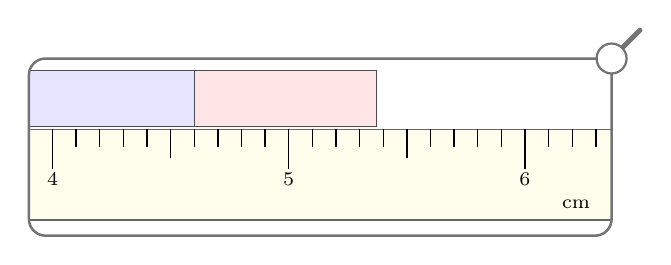
\begin{tikzpicture}
  \zoomclip{-3.3}{-1.35}{4.1}{0.9}
    \filldraw[fill=blue!10, draw=black!70] (-5,0.04) rectangle (-1.2,0.75);
    \filldraw[fill=red!10, draw=black!70] (-1.2,0.04) rectangle (1.11,0.75);
    \filldraw[scalebody] (-5,-1.15) rectangle (6,0);
    \hticks{-12}{15}{0.3}{10}{5}{5}{0.1}
    \node[ticklab] at (3.65,-0.95) {cm};
  \zoomframe
\end{tikzpicture}}
{One \ealkey{gap} is worth \ansline[0.9cm]\,mm, which is \ansline[0.9cm]\,cm.\\[4pt]
\ealkey{Reading} to the nearest \ealkey{tick}: \ansline[1.3cm]\,cm.}

\vfill
% Q7: pointer at 23.66 kg. The values increase downwards, so
% y = -(23.66 - 23) / 0.2 * 0.5 = -1.65.
\ealpara{Walizkę waży się na wadze bagażowej. Liczby na tej wadze rosną w dół. Jeden \ealkeytr{odstęp} jest wart ... kg. \ealkeytr{Odczyt} do najbliższej \ealkeytr{kreski}: ... kg.}{}
\vcell{\q A suitcase is weighed with luggage scales. The numbers on these
scales increase downwards.}
{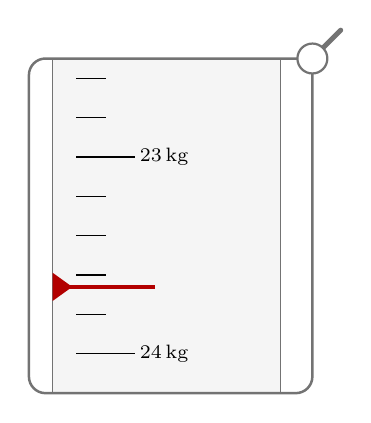
\begin{tikzpicture}[baseline=(current bounding box.north)]
  \zoomclip{-0.6}{-3.0}{3.0}{1.25}
    \filldraw[fill=black!4, draw=black!55] (-0.3,-5) rectangle (2.6,3);
    \vticks{-3}{7}{-0.5}{5}{100}{23}{0.2}{kg}
    \draw[red!70!black, line width=1.2pt] (-0.3,-1.65) -- (1.0,-1.65);
    \fill[red!70!black] (-0.3,-1.47) -- (-0.05,-1.65) -- (-0.3,-1.83) -- cycle;
  \zoomframe
\end{tikzpicture}}
{One \ealkey{gap} is worth \ansline[1.3cm]\,kg.\\[8pt]
\ealkey{Reading} to the nearest \ealkey{tick}:\\[4pt] \ansline[1.6cm]\,kg.}%
\hfill
% Q8: surface of the river at 1.27 m, so y = 2.7 * 0.4 = 1.08.
\ealpara{Wskaźnik \ealkeytr{głębokości} to słupek, który stoi na dnie rzeki i jest oznaczony w metrach. Pokazuje \ealkeytr{głębokość} wody. \ealkeytr{Odczyt} do najbliższej \ealkeytr{kreski}: ... m.}{}
\vcell{\q A \ealkey{depth} gauge is a post that stands on the river bed and is marked
in metres. It shows the \ealkey{depth} of the water.}
{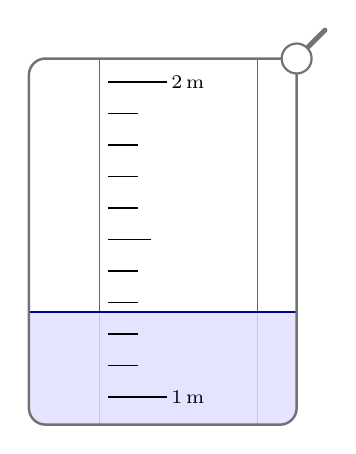
\begin{tikzpicture}[baseline=(current bounding box.north)]
  \zoomclip{-1.0}{-0.35}{2.4}{4.3}
    \filldraw[fill=white, draw=black!60] (-0.1,-2) rectangle (1.9,6);
    \fill[water, fill opacity=0.8] (-2,-2) rectangle (3,1.08);
    \vticks{-2}{11}{0.4}{10}{5}{1}{0.1}{m}
    \draw[surface] (-2,1.08) -- (3,1.08);
  \zoomframe
\end{tikzpicture}}
{\ealkey{Reading} to the nearest \ealkey{tick}:\\[4pt] \ansline[1.6cm]\,m.}

\newpage
\ealpara{2 \ealkeytr{Przedziały błędu}}{}
\parttitle{2}{\ealkey{Error intervals}}

\begin{keyidea}
\ealpara{Kiedy odczytujemy skalę do najbliższej \ealkeytr{kreski}, \ealkeytr{odczyt} nie jest \ealkeytr{ścisłym} \ealkeytr{pomiarem}. Prawdziwy \ealkeytr{pomiar} może być do połowy jednego \ealkeytr{odstępu} poniżej \ealkeytr{odczytu} albo do połowy jednego \ealkeytr{odstępu} powyżej niego. Na metrze oznaczonym w centymetrach jeden \ealkeytr{odstęp} wynosi 1\,cm, więc \ealkeytr{odczyt} 73\,cm jest \ealkeytr{dokładny} do $\pm\,0.5$\,cm. Symbol $\pm$ oznacza „\ealkeytr{plus minus}”.}{When we read a scale to the nearest \ealkey{tick}, the \ealkey{reading} is not the \ealkey{exact} \ealkey{measurement}. The true \ealkey{measurement} could be up to half of one \ealkey{gap} below the \ealkey{reading}, or up to half of one \ealkey{gap} above it. On a metre rule marked in centimetres one \ealkey{gap} is 1\,cm, so a \ealkey{reading} of 73\,cm is \ealkey{accurate} to $\pm\,0.5$\,cm. The symbol $\pm$ means ``\ealkey{plus or minus}''.}

\smallskip
\ealpara{Najmniejszą wartością, jaką prawdziwy \ealkeytr{pomiar} mógłby być, jest \ealkeytr{dolna granica}. Prawdziwy \ealkeytr{pomiar} musi być mniejszy niż \ealkeytr{ograniczenie górne}: \ealkeytr{długość} wynosząca \ealkeytr{ściśle} 73.5\,cm leży w połowie między dwiema \ealkeytr{kreskami}, a wartości w połowie są \ealkeytr{zaokrąglane w górę}, więc zostałaby odczytana jako 74\,cm.}{The smallest value the true \ealkey{measurement} could be is the \textbf{\ealkey{lower bound}}. The true \ealkey{measurement} must be less than the \textbf{\ealkey{upper bound}}: a \ealkey{length} of \ealkey{exactly} 73.5\,cm is halfway between two \ealkey{ticks}, and halfway values are \ealkey{rounded up}, so it would be read as 74\,cm.}

\smallskip
\ealpara{\ealkeytr{Przedział błędu} podaje każdą wartość, jaką prawdziwy \ealkeytr{pomiar} mógłby być. Zapisujemy go za pomocą symboli \ealkeytr{nierówności} $\le$, co oznacza „jest mniejsze lub równe”, oraz $<$, co oznacza „jest mniejsze”.}{The \textbf{\ealkey{error interval}} gives every value the true \ealkey{measurement} could be. We write it with the \ealkey{inequality} symbols $\le$, which means ``is less than or equal to'', and $<$, which means ``is less than''.}
\end{keyidea}

\ealpara{Przykład: linijka metrowa oznaczona w centymetrach}{}
\begin{wex}{a metre rule marked in centimetres}
\ealpara{Stół mierzy się metrem oznaczonym w centymetrach. \ealkeytr{Odczyt} do najbliższej \ealkeytr{kreski} wynosi 73\,cm.}{A table is measured with a metre rule marked in centimetres. The \ealkey{reading} to the nearest \ealkey{tick} is 73\,cm.}

\smallskip
\ealpara{Nagłówki tabeli: \ealkeytr{Odczyt} do najbliższej \ealkeytr{kreski}; \ealkeytr{Odstęp} między dwiema \ealkeytr{kreskami}; Połowa \ealkeytr{odstępu}; \ealkeytr{Dolna granica}; \ealkeytr{Ograniczenie górne}; \ealkeytr{Przedział błędu}.}{}
\begin{minipage}[t]{0.61\linewidth}\vspace{0pt}
\renewcommand{\arraystretch}{1.4}
\begin{tabular}{@{}ll@{}}
\ealkey{Reading} to the nearest \ealkey{tick} & 73\,cm\\
\ealkey{Gap} between two \ealkey{ticks} & 1\,cm\\
Half of the \ealkey{gap} & $1\div2=0.5$\,cm\\
\ealkey{Lower bound} & $73-0.5=72.5$\,cm\\
\ealkey{Upper bound} & $73+0.5=73.5$\,cm\\
\ealkey{Error interval} & $72.5\,\text{cm}\le\text{\ealkey{length}}<73.5\,\text{cm}$
\end{tabular}
\end{minipage}\hfill
\begin{minipage}[t]{0.38\linewidth}\vspace{14pt}
\centering
\numline{72\,cm}{73\,cm}{74\,cm}{%
  \draw[densely dashed, black!55] (0.5,-0.15) -- (0.5,0.55);
  \draw[densely dashed, black!55] (1.5,-0.15) -- (1.5,0.55);
  \draw[line width=3.5pt, blue!25] (0.5,0) -- (1.5,0);
  \fill[blue!55!black] (0.5,0) circle (2.5pt);
  \draw[blue!55!black, line width=1pt, fill=white] (1.5,0) circle (2.5pt);
  \node[ticklab, above, align=center] at (0.5,0.55) {lower bound\\72.5\,cm};
  \node[ticklab, above, align=center] at (1.5,0.55) {upper bound\\73.5\,cm};
  \draw[decorate, decoration={brace, mirror, amplitude=3pt}] (0.52,-0.62) -- (0.98,-0.62)
    node[midway, below=3pt, ticklab] {0.5\,cm};
  \draw[decorate, decoration={brace, mirror, amplitude=3pt}] (1.02,-0.62) -- (1.48,-0.62)
    node[midway, below=3pt, ticklab] {0.5\,cm};}

\smallskip
{\scriptsize
\ealpara{\ealkeytr{Wypełnione kółko} pokazuje, że 72.5\,cm jest uwzględnione.}{The \ealkey{filled circle} shows that 72.5\,cm is included.}
\ealpara{\ealkeytr{Puste kółko} pokazuje, że 73.5\,cm nie jest uwzględnione.}{The \ealkey{open circle} shows that 73.5\,cm is not included.}
}
\end{minipage}
\end{wex}

\begin{enumerate}\setcounter{enumi}{\value{qn}}
\item \ealpara{Półkę mierzy się metrem oznaczonym w centymetrach. \ealkeytr{Odczyt} do najbliższej \ealkeytr{kreski} wynosi 48\,cm. Uzupełnij obliczenia, aby znaleźć \ealkeytr{przedział błędu}, a następnie pokaż \ealkeytr{przedział błędu} na \ealkeytr{osi liczbowej}.}{A shelf is measured with a metre rule marked in centimetres. The \ealkey{reading}
to the nearest \ealkey{tick} is 48\,cm. Complete the working to find the \ealkey{error interval},
then show the \ealkey{error interval} on the \ealkey{number line}.}

\smallskip
\ealpara{Wiersze tabeli: \ealkeytr{Odczyt} do najbliższej \ealkeytr{kreski} = 48\,cm; \ealkeytr{Odstęp} między dwiema \ealkeytr{kreskami} = ...; Połowa \ealkeytr{odstępu} = ...; \ealkeytr{Dolna granica} = ...; \ealkeytr{Ograniczenie górne} = ...; \ealkeytr{Przedział błędu} = ... $\le$ \ealkeytr{długość} $<$ ...}{}
\begin{minipage}[t]{0.61\linewidth}\vspace{0pt}
\renewcommand{\arraystretch}{1.6}
\begin{tabular}{@{}ll@{}}
\ealkey{Reading} to the nearest \ealkey{tick} & 48\,cm\\
\ealkey{Gap} between two \ealkey{ticks} & \ansline[1.1cm]\,cm\\
Half of the \ealkey{gap} & \ansline[1.1cm]${}\div2={}$\ansline[1.1cm]\,cm\\
\ealkey{Lower bound} & $48-{}$\ansline[1.1cm]${}={}$\ansline[1.1cm]\,cm\\
\ealkey{Upper bound} & $48+{}$\ansline[1.1cm]${}={}$\ansline[1.1cm]\,cm\\
\ealkey{Error interval} & \ansline[1.1cm]\,cm $\le$ \ealkey{length} $<$ \ansline[1.1cm]\,cm
\end{tabular}
\end{minipage}\hfill
\begin{minipage}[t]{0.38\linewidth}\vspace{30pt}
\centering
\numline{47\,cm}{48\,cm}{49\,cm}{}
\end{minipage}

\item \ealpara{Wodę wlewa się do dzbanka miarowego oznaczonego co 20\,ml. \ealkeytr{Odczyt} do najbliższej \ealkeytr{kreski} wynosi 180\,ml. Znajdź \ealkeytr{przedział błędu}, a następnie pokaż go na \ealkeytr{osi liczbowej}.}{Water is poured into a measuring jug marked every 20\,ml. The \ealkey{reading} to
the nearest \ealkey{tick} is 180\,ml. Find the \ealkey{error interval}, then show it on the
\ealkey{number line}.}

\smallskip
\ealpara{Wiersze tabeli: \ealkeytr{Odczyt} do najbliższej \ealkeytr{kreski} = 180\,ml; \ealkeytr{Odstęp} między dwiema \ealkeytr{kreskami} = ...; Połowa \ealkeytr{odstępu} = ...; \ealkeytr{Dolna granica} = ...; \ealkeytr{Ograniczenie górne} = ...; \ealkeytr{Przedział błędu} dla \ealkeytr{objętości} = ... $\le$ ... $<$ ...}{}
\begin{minipage}[t]{0.61\linewidth}\vspace{0pt}
\renewcommand{\arraystretch}{1.6}
\begin{tabular}{@{}ll@{}}
\ealkey{Reading} to the nearest \ealkey{tick} & 180\,ml\\
\ealkey{Gap} between two \ealkey{ticks} & \ansline[3.6cm]\\
Half of the \ealkey{gap} & \ansline[3.6cm]\\
\ealkey{Lower bound} & \ansline[3.6cm]\\
\ealkey{Upper bound} & \ansline[3.6cm]\\
\ealkey{Error interval} & \ansline[1.1cm]\,ml $\le$ \ealkey{volume} $<$ \ansline[1.1cm]\,ml
\end{tabular}
\end{minipage}\hfill
\begin{minipage}[t]{0.38\linewidth}\vspace{30pt}
\centering
\numline{160\,ml}{180\,ml}{200\,ml}{}
\end{minipage}

\item \ealpara{Wróć do części 1. Zapisz \ealkeytr{przedział błędu} dla każdego z tych \ealkeytr{odczytów}.}{Go back to Part 1. Write the \ealkey{error interval} for each of these \ealkey{readings}.}

\smallskip
\ealpara{W nierównościach: \ealkeytr{długość} (Q1, Q6), \ealkeytr{objętość} (Q3), \ealkeytr{masa} (Q7).}{}
\renewcommand{\arraystretch}{1.7}
\begin{tabular}{@{}l@{\ \ }l@{\qquad\quad}l@{\ \ }l@{}}
Q1: & \ansline[1.5cm]\,cm $\le$ \ealkey{length} $<$ \ansline[1.5cm]\,cm &
Q3: & \ansline[1.5cm]\,ml $\le$ \ealkey{volume} $<$ \ansline[1.5cm]\,ml\\
Q6: & \ansline[1.5cm]\,cm $\le$ \ealkey{length} $<$ \ansline[1.5cm]\,cm &
Q7: & \ansline[1.5cm]\,kg $\le$ \ealkey{mass} $<$ \ansline[1.5cm]\,kg
\end{tabular}

\newpage
\item \ealpara{Uzupełnij tabelę. Pierwsza kolumna mówi, co jest mierzone oraz jak daleko od siebie są \ealkeytr{kreski} na skali, która jest używana.}{Complete the table. The first column says what is measured, and how far
apart the \ealkey{ticks} are on the scale that is used.}

\smallskip
\ealpara{Nagłówki tabeli: Co jest mierzone; \ealkeytr{Odczyt}; Połowa \ealkeytr{odstępu}; \ealkeytr{Dolna granica}; \ealkeytr{Ograniczenie górne}; \ealkeytr{Przedział błędu}. Wiersze: Ołówek, linijką oznaczoną co 1\,cm; Chrząszcz, linijką oznaczoną co 1\,mm; Torba mąki, wagą kuchenną oznaczoną co 10\,g; \ealkeytr{Wysokość} ucznia, miarką \ealkeytr{wysokości} oznaczoną co 2\,cm; Sok pomarańczowy, dzbankiem oznaczonym co 50\,ml; Paczka, wagą oznaczoną co 0.2\,kg; Lek, strzykawką oznaczoną co 0.5\,ml; Ogród, taśmą mierniczą oznaczoną co 10\,cm.}{}
{\small
\setlength{\tabcolsep}{3pt}
\begin{tabular}{|>{\raggedright\arraybackslash}m{5.0cm}|C{1.4cm}|C{1.45cm}|C{1.45cm}|C{1.45cm}|C{4.65cm}|}
\hline
\textbf{What is measured} & \textbf{\ealkey{Reading}} & \textbf{Half of the \ealkey{gap}} & \textbf{\ealkey{Lower bound}} & \textbf{\ealkey{Upper bound}} & \textbf{\ealkey{Error interval}}\\\hline
A pencil, with a ruler marked every 1\,cm & 15\,cm\rowstrut & & & & \\\hline
A beetle, with a ruler marked every 1\,mm & 23\,mm\rowstrut & & & & \\\hline
A bag of flour, with kitchen scales marked every 10\,g & 510\,g\rowstrut & & & & \\\hline
A pupil's \ealkey{height}, with a \ealkey{height} chart marked every 2\,cm & 148\,cm\rowstrut & & & & \\\hline
Orange juice, with a jug marked every 50\,ml & 250\,ml\rowstrut & & & & \\\hline
A parcel, with scales marked every 0.2\,kg & 3.4\,kg\rowstrut & & & & \\\hline
Medicine, with a syringe marked every 0.5\,ml & 2.5\,ml\rowstrut & & & & \\\hline
A garden, with a tape measure marked every 10\,cm & 12.4\,m\rowstrut & & & & \\\hline
\end{tabular}}
\end{enumerate}

\ealpara{3 Używanie \ealkeytr{przedziałów błędu}}{}
\parttitle{3}{Using \ealkey{error intervals}}

\begin{enumerate}[resume]
\item \ealpara{Każdy poniższy \ealkeytr{przedział błędu} pochodzi z \ealkeytr{odczytu} do najbliższej \ealkeytr{kreski}. Znajdź \ealkeytr{odczyt} oraz znajdź \ealkeytr{odstęp} między dwiema \ealkeytr{kreskami} na skali, która została użyta.}{Each \ealkey{error interval} below comes from a \ealkey{reading} to the nearest \ealkey{tick}. Find
the \ealkey{reading}, and find the \ealkey{gap} between two \ealkey{ticks} on the scale that was used.}

\smallskip
\ealpara{W tabeli: \ealkeytr{Odczyt}; \ealkeytr{Odstęp}; oraz w nierównościach: \ealkeytr{długość}, \ealkeytr{masa}, \ealkeytr{wysokość}.}{}
\renewcommand{\arraystretch}{1.8}
\begin{tabular}{@{}l@{\qquad}l@{\qquad}l@{}}
(a) $30.5\,\text{cm}\le\text{\ealkey{length}}<31.5\,\text{cm}$ & \ealkey{Reading}: \ansline[1.8cm] & \ealkey{Gap}: \ansline[1.8cm]\\
(b) $245\,\text{g}\le\text{\ealkey{mass}}<255\,\text{g}$ & \ealkey{Reading}: \ansline[1.8cm] & \ealkey{Gap}: \ansline[1.8cm]\\
(c) $1.35\,\text{m}\le\text{\ealkey{height}}<1.45\,\text{m}$ & \ealkey{Reading}: \ansline[1.8cm] & \ealkey{Gap}: \ansline[1.8cm]
\end{tabular}

\item \ealpara{Leo waży swoją walizkę na wadze bagażowej oznaczoną co 0.2\,kg. \ealkeytr{Odczyt} wynosi 23.0\,kg. Jego linia lotnicza pozwala na walizki o \ealkeytr{masie} 23\,kg lub mniejszej. Czy Leo może być pewien, że jego walizka jest dozwolona? Wyjaśnij, używając \ealkeytr{przedziału błędu}.}{Leo weighs his suitcase with luggage scales marked every 0.2\,kg. The
\ealkey{reading} is 23.0\,kg. His airline allows suitcases with a \ealkey{mass} of 23\,kg or
less. Can Leo be sure that his suitcase is allowed? Explain using the \ealkey{error
interval}.}
\wline\wline\wline

\item \ealpara{Sam mierzy liść linijką oznaczoną w milimetrach. Sam mówi: „\ealkeytr{Kreski} na mojej linijce są bardzo blisko siebie, więc liść ma \ealkeytr{ściśle} 6.3\,cm długości.” Czy Sam ma rację? Wyjaśnij.}{Sam measures a leaf with a ruler marked in millimetres. Sam says, ``The
\ealkey{ticks} on my ruler are very close together, so the leaf is \ealkey{exactly} 6.3\,cm
long.'' Is Sam right? Explain.}
\wline\wline\wline

\newpage
\item \ealpara{Przepis na ciastka działa, jeśli \ealkeytr{masa} masła wynosi \ealkeytr{co najmniej} 195\,g i mniej niż 205\,g. Kucharz dodaje masło do miski, aż waga pokaże 200\,g. Waga A jest oznaczona co 10\,g. Waga B jest oznaczona co 50\,g.}{A biscuit recipe works if the \ealkey{mass} of butter is \ealkey{at least} 195\,g and less
than 205\,g. A chef adds butter to a bowl until the scales read 200\,g. Scales
A are marked every 10\,g. Scales B are marked every 50\,g.}
\begin{enumerate}
\item \ealpara{Napisz \ealkeytr{przedział błędu} dla \ealkeytr{odczytu} 200\,g na wadze A. (W nierówności: \ealkeytr{masa}.)}{Write the \ealkey{error interval} for the \ealkey{reading} of 200\,g on scales A.}
\smallskip
\ansline[1.6cm]\,g $\le$ \ealkey{mass} $<$ \ansline[1.6cm]\,g
\item \ealpara{Napisz \ealkeytr{przedział błędu} dla \ealkeytr{odczytu} 200\,g na wadze B. (W nierówności: \ealkeytr{masa}.)}{Write the \ealkey{error interval} for the \ealkey{reading} of 200\,g on scales B.}
\smallskip
\ansline[1.6cm]\,g $\le$ \ealkey{mass} $<$ \ansline[1.6cm]\,g
\item \ealpara{Której wagi powinien użyć kucharz? Wyjaśnij.}{Which scales should the chef use? Explain.}
\wline\wline
\end{enumerate}

\newpage
\item \begin{minipage}[t]{0.68\linewidth}
\ealpara{Narysuj \ealkeytr{kreski} na pustej skali tego dzbanka miarowego tak, aby \ealkeytr{odczyt} 300\,ml miał \ealkeytr{przedział błędu} dla \ealkeytr{objętości}}{Draw \ealkey{ticks} on the empty scale of this measuring jug so that a \ealkey{reading} of
300\,ml has the \ealkey{error interval}}
\[295\,\text{ml}\le\text{\ealkey{volume}}<305\,\text{ml}.\]
\ealpara{\ealkeytr{Kreska} dla 300\,ml została narysowana za ciebie. Oznacz \ealkeytr{co najmniej} dwie kolejne \ealkeytr{kreski}.}{The \ealkey{tick} for 300\,ml has been drawn for you. Label \ealkey{at least} two more \ealkey{ticks}.}

\medskip
\ealpara{Wyjaśnij, jak wybrałeś \ealkeytr{odstęp} między \ealkeytr{kreskami}.}{Explain how you chose the \ealkey{gap} between the \ealkey{ticks}.}
\wline\wline
\end{minipage}\hfill
\begin{minipage}[t]{0.27\linewidth}
\centering
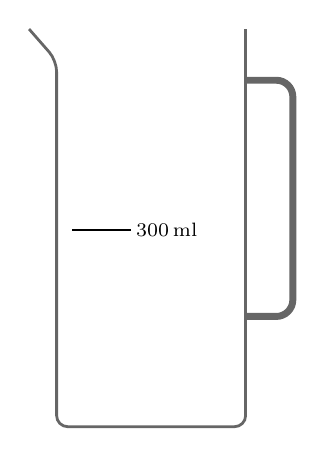
\begin{tikzpicture}[baseline=(current bounding box.north)]
  % The jug: a spout at the top left and a handle on the right.
  \draw[black!60, line width=1pt, rounded corners=4pt]
    (-0.35,5.05) -- (0,4.65) -- (0,0) -- (2.4,0) -- (2.4,5.05);
  \draw[black!60, line width=2.5pt, rounded corners=6pt]
    (2.4,4.4) -- (3.0,4.4) -- (3.0,1.4) -- (2.4,1.4);
  \draw[tick] (0.2,2.5) -- ++(0.75,0);
  \node[ticklab,right] at (0.95,2.5) {300\,ml};
\end{tikzpicture}
\end{minipage}

\item \ealpara{\textbf{Wyzwanie.} Ana mierzy półkę metrem oznaczonym w centymetrach, a \ealkeytr{odczyt} wynosi 80\,cm. Mierzy \ealkeytr{odstęp} między dwiema ścianami tym samym metrem, a \ealkeytr{odczyt} również wynosi 80\,cm. Czy półka na pewno zmieści się w \ealkeytr{odstępie}? Wyjaśnij, używając \ealkeytr{przedziałów błędu}.}{\textbf{Challenge.} Ana measures a shelf with a metre rule marked in
centimetres, and the \ealkey{reading} is 80\,cm. She measures the \ealkey{gap} between two walls
with the same metre rule, and the \ealkey{reading} is also 80\,cm. Will the shelf
definitely fit in the \ealkey{gap}? Explain using \ealkey{error intervals}.}
\wline\wline\wline\wline

\item \ealpara{Wybierz przyrząd pomiarowy w domu lub w szkole, taki jak waga łazienkowa, łyżka miarowa lub taśma miernicza.}{Choose a measuring instrument at home or at school, such as bathroom
scales, a measuring spoon or a tape measure.}
\begin{enumerate}
\item \ealpara{Nazwij przyrząd i powiedz, jak daleko od siebie są \ealkeytr{kreski} na jego skali.}{Name the instrument, and say how far apart the \ealkey{ticks} on its scale are.}
\wline
\item \ealpara{Wymyśl \ealkeytr{odczyt} na tej skali i zapisz jego \ealkeytr{przedział błędu}.}{Make up a \ealkey{reading} on this scale, and write its \ealkey{error interval}.}
\wline
\item \ealpara{Opisz jedno zadanie, do którego ten przyrząd jest wystarczająco \ealkeytr{dokładny}, oraz jedno zadanie, do którego nie jest wystarczająco \ealkeytr{dokładny}. Wyjaśnij, używając \ealkeytr{przedziału błędu}.}{Describe one job that this instrument is \ealkey{accurate} enough for, and one
job that it is not \ealkey{accurate} enough for. Explain using the \ealkey{error interval}.}
\wline\wline\wline
\end{enumerate}
\end{enumerate}

\end{document}